\documentclass{article}
\usepackage{amsmath}
\usepackage{tikz}
\usepackage{hyperref}
\usetikzlibrary{positioning}
\newcommand\abs[1]{\left|#1\right|}

\begin{document}

\title{%
  Introduction to Graph Theory \\
  \large by Richard Trudeau \\
   Ch. 3 Solutions}
   \author{Tyler Bailey}
\maketitle

\begin{enumerate}
	\item[1] Prove the following statements:
	
	\begin{enumerate}
		\item[a] If 3 edges were added to the graph in Figure 63a, then at least 2 of the new edges will be adjacent.
		\item[b] Every graph with $v = 5$ and $e = 3$ has at least two adjacent edges.
		\item[c] If $v$ is an odd number, then every graph with $v$ vertices and $\frac{1}{2}(v + 1)$ edges has at least two adjacent edges.
	\end{enumerate}
	
	\textbf{Solution:}
	\begin{enumerate}
		\item[a] This is a straightforward application of the pigeonhole principle. If we add one edge, we connect two vertices. If we add another vertex it will either touch an existing vertex (and we are done) or not. If not, then we now have 4 vertices connected, none of which have adjacent edges, and one isolated vertex. For the final edge, no matter how we attach it, it must be adjacent to at least one other edge.
		\item[b] We proved this in item $a$ because we did not utilize the fact that Figure 63a was $C_5$.
		\item[c] This follows by the same pigeonhole argument as the previous two items. If we attach $\frac{1}{2}(v - 1)$ edges, we either have adjacent edges already, or we don't. If we don't, then we have connected a single isolated vertex and a final edge to add. Therefore, any connection will create two adjacent edges.
	\end{enumerate}
	\item[2] Prove that in Figure 58, graph a) is planar, and graphs b) and c) are non-planar.
	
	\textbf{Solution:}
		\begin{enumerate}
			\item[a] This graph is isomorphic to the following planar graph:
			
				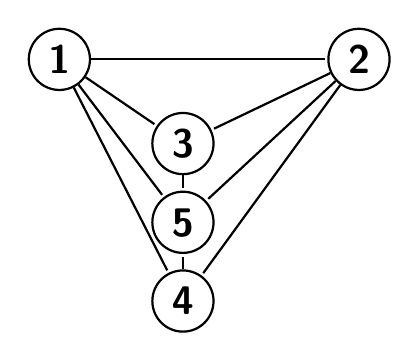
\begin{tikzpicture}[shorten >=1pt,auto,node distance=3cm,
                    thick,main node/.style={circle,draw,font=\sffamily\Large\bfseries}]
                    	\node[main node] (1) {1};
                    	\node[main node] (2) [right=3cm of 1] {2};
                    	\node[main node] (3) [below right=0.5cm and 1cm of 1] {3};
                    	\node[main node] (5) [below right=1.5cm and 1cm of 1] {5};
					\node[main node] (4) [below right=2.5cm and 1cm of 1] {4};

                    \path[every node/.style={font=\sffamily\small}]
             		(1)	edge node [left] {} (2)
                    		edge node [left] {} (3)
                    		edge node [left] {} (4)
						edge node [left] {} (5)
                 	(2)	edge node [right] {} (3)
                 		edge node [right] {} (4)
                 		edge node [right] {} (5)
                 	(3)	edge node [right] {} (5)
					(4)	edge node [right] {} (5);

				\end{tikzpicture}
			\item[b] This is a supergraph of $UG$.
			\item[c] $K_7$ is a supergraph of $K_5$.
			\end{enumerate}
\end{enumerate}

\end{document}